% Options for packages loaded elsewhere
\PassOptionsToPackage{unicode}{hyperref}
\PassOptionsToPackage{hyphens}{url}
\PassOptionsToPackage{dvipsnames,svgnames,x11names}{xcolor}
%
\documentclass[
  letterpaper,
  DIV=11,
  numbers=noendperiod]{scrartcl}

\usepackage{amsmath,amssymb}
\usepackage{lmodern}
\usepackage{iftex}
\ifPDFTeX
  \usepackage[T1]{fontenc}
  \usepackage[utf8]{inputenc}
  \usepackage{textcomp} % provide euro and other symbols
\else % if luatex or xetex
  \usepackage{unicode-math}
  \defaultfontfeatures{Scale=MatchLowercase}
  \defaultfontfeatures[\rmfamily]{Ligatures=TeX,Scale=1}
\fi
% Use upquote if available, for straight quotes in verbatim environments
\IfFileExists{upquote.sty}{\usepackage{upquote}}{}
\IfFileExists{microtype.sty}{% use microtype if available
  \usepackage[]{microtype}
  \UseMicrotypeSet[protrusion]{basicmath} % disable protrusion for tt fonts
}{}
\makeatletter
\@ifundefined{KOMAClassName}{% if non-KOMA class
  \IfFileExists{parskip.sty}{%
    \usepackage{parskip}
  }{% else
    \setlength{\parindent}{0pt}
    \setlength{\parskip}{6pt plus 2pt minus 1pt}}
}{% if KOMA class
  \KOMAoptions{parskip=half}}
\makeatother
\usepackage{xcolor}
\setlength{\emergencystretch}{3em} % prevent overfull lines
\setcounter{secnumdepth}{-\maxdimen} % remove section numbering
% Make \paragraph and \subparagraph free-standing
\ifx\paragraph\undefined\else
  \let\oldparagraph\paragraph
  \renewcommand{\paragraph}[1]{\oldparagraph{#1}\mbox{}}
\fi
\ifx\subparagraph\undefined\else
  \let\oldsubparagraph\subparagraph
  \renewcommand{\subparagraph}[1]{\oldsubparagraph{#1}\mbox{}}
\fi

\usepackage{color}
\usepackage{fancyvrb}
\newcommand{\VerbBar}{|}
\newcommand{\VERB}{\Verb[commandchars=\\\{\}]}
\DefineVerbatimEnvironment{Highlighting}{Verbatim}{commandchars=\\\{\}}
% Add ',fontsize=\small' for more characters per line
\usepackage{framed}
\definecolor{shadecolor}{RGB}{241,243,245}
\newenvironment{Shaded}{\begin{snugshade}}{\end{snugshade}}
\newcommand{\AlertTok}[1]{\textcolor[rgb]{0.68,0.00,0.00}{#1}}
\newcommand{\AnnotationTok}[1]{\textcolor[rgb]{0.37,0.37,0.37}{#1}}
\newcommand{\AttributeTok}[1]{\textcolor[rgb]{0.40,0.45,0.13}{#1}}
\newcommand{\BaseNTok}[1]{\textcolor[rgb]{0.68,0.00,0.00}{#1}}
\newcommand{\BuiltInTok}[1]{\textcolor[rgb]{0.00,0.23,0.31}{#1}}
\newcommand{\CharTok}[1]{\textcolor[rgb]{0.13,0.47,0.30}{#1}}
\newcommand{\CommentTok}[1]{\textcolor[rgb]{0.37,0.37,0.37}{#1}}
\newcommand{\CommentVarTok}[1]{\textcolor[rgb]{0.37,0.37,0.37}{\textit{#1}}}
\newcommand{\ConstantTok}[1]{\textcolor[rgb]{0.56,0.35,0.01}{#1}}
\newcommand{\ControlFlowTok}[1]{\textcolor[rgb]{0.00,0.23,0.31}{#1}}
\newcommand{\DataTypeTok}[1]{\textcolor[rgb]{0.68,0.00,0.00}{#1}}
\newcommand{\DecValTok}[1]{\textcolor[rgb]{0.68,0.00,0.00}{#1}}
\newcommand{\DocumentationTok}[1]{\textcolor[rgb]{0.37,0.37,0.37}{\textit{#1}}}
\newcommand{\ErrorTok}[1]{\textcolor[rgb]{0.68,0.00,0.00}{#1}}
\newcommand{\ExtensionTok}[1]{\textcolor[rgb]{0.00,0.23,0.31}{#1}}
\newcommand{\FloatTok}[1]{\textcolor[rgb]{0.68,0.00,0.00}{#1}}
\newcommand{\FunctionTok}[1]{\textcolor[rgb]{0.28,0.35,0.67}{#1}}
\newcommand{\ImportTok}[1]{\textcolor[rgb]{0.00,0.46,0.62}{#1}}
\newcommand{\InformationTok}[1]{\textcolor[rgb]{0.37,0.37,0.37}{#1}}
\newcommand{\KeywordTok}[1]{\textcolor[rgb]{0.00,0.23,0.31}{#1}}
\newcommand{\NormalTok}[1]{\textcolor[rgb]{0.00,0.23,0.31}{#1}}
\newcommand{\OperatorTok}[1]{\textcolor[rgb]{0.37,0.37,0.37}{#1}}
\newcommand{\OtherTok}[1]{\textcolor[rgb]{0.00,0.23,0.31}{#1}}
\newcommand{\PreprocessorTok}[1]{\textcolor[rgb]{0.68,0.00,0.00}{#1}}
\newcommand{\RegionMarkerTok}[1]{\textcolor[rgb]{0.00,0.23,0.31}{#1}}
\newcommand{\SpecialCharTok}[1]{\textcolor[rgb]{0.37,0.37,0.37}{#1}}
\newcommand{\SpecialStringTok}[1]{\textcolor[rgb]{0.13,0.47,0.30}{#1}}
\newcommand{\StringTok}[1]{\textcolor[rgb]{0.13,0.47,0.30}{#1}}
\newcommand{\VariableTok}[1]{\textcolor[rgb]{0.07,0.07,0.07}{#1}}
\newcommand{\VerbatimStringTok}[1]{\textcolor[rgb]{0.13,0.47,0.30}{#1}}
\newcommand{\WarningTok}[1]{\textcolor[rgb]{0.37,0.37,0.37}{\textit{#1}}}

\providecommand{\tightlist}{%
  \setlength{\itemsep}{0pt}\setlength{\parskip}{0pt}}\usepackage{longtable,booktabs,array}
\usepackage{calc} % for calculating minipage widths
% Correct order of tables after \paragraph or \subparagraph
\usepackage{etoolbox}
\makeatletter
\patchcmd\longtable{\par}{\if@noskipsec\mbox{}\fi\par}{}{}
\makeatother
% Allow footnotes in longtable head/foot
\IfFileExists{footnotehyper.sty}{\usepackage{footnotehyper}}{\usepackage{footnote}}
\makesavenoteenv{longtable}
\usepackage{graphicx}
\makeatletter
\def\maxwidth{\ifdim\Gin@nat@width>\linewidth\linewidth\else\Gin@nat@width\fi}
\def\maxheight{\ifdim\Gin@nat@height>\textheight\textheight\else\Gin@nat@height\fi}
\makeatother
% Scale images if necessary, so that they will not overflow the page
% margins by default, and it is still possible to overwrite the defaults
% using explicit options in \includegraphics[width, height, ...]{}
\setkeys{Gin}{width=\maxwidth,height=\maxheight,keepaspectratio}
% Set default figure placement to htbp
\makeatletter
\def\fps@figure{htbp}
\makeatother

<script src="k-means_final_files/libs/htmlwidgets-1.6.2/htmlwidgets.js"></script>
<script src="k-means_final_files/libs/plotly-binding-4.10.1/plotly.js"></script>
<script src="k-means_final_files/libs/setprototypeof-0.1/setprototypeof.js"></script>
<script src="k-means_final_files/libs/typedarray-0.1/typedarray.min.js"></script>
<script src="k-means_final_files/libs/jquery-3.5.1/jquery.min.js"></script>
<link href="k-means_final_files/libs/crosstalk-1.2.0/css/crosstalk.min.css" rel="stylesheet" />
<script src="k-means_final_files/libs/crosstalk-1.2.0/js/crosstalk.min.js"></script>
<link href="k-means_final_files/libs/plotly-htmlwidgets-css-2.11.1/plotly-htmlwidgets.css" rel="stylesheet" />
<script src="k-means_final_files/libs/plotly-main-2.11.1/plotly-latest.min.js"></script>
\KOMAoption{captions}{tableheading}
\makeatletter
\makeatother
\makeatletter
\makeatother
\makeatletter
\@ifpackageloaded{caption}{}{\usepackage{caption}}
\AtBeginDocument{%
\ifdefined\contentsname
  \renewcommand*\contentsname{Table of contents}
\else
  \newcommand\contentsname{Table of contents}
\fi
\ifdefined\listfigurename
  \renewcommand*\listfigurename{List of Figures}
\else
  \newcommand\listfigurename{List of Figures}
\fi
\ifdefined\listtablename
  \renewcommand*\listtablename{List of Tables}
\else
  \newcommand\listtablename{List of Tables}
\fi
\ifdefined\figurename
  \renewcommand*\figurename{Figure}
\else
  \newcommand\figurename{Figure}
\fi
\ifdefined\tablename
  \renewcommand*\tablename{Table}
\else
  \newcommand\tablename{Table}
\fi
}
\@ifpackageloaded{float}{}{\usepackage{float}}
\floatstyle{ruled}
\@ifundefined{c@chapter}{\newfloat{codelisting}{h}{lop}}{\newfloat{codelisting}{h}{lop}[chapter]}
\floatname{codelisting}{Listing}
\newcommand*\listoflistings{\listof{codelisting}{List of Listings}}
\makeatother
\makeatletter
\@ifpackageloaded{caption}{}{\usepackage{caption}}
\@ifpackageloaded{subcaption}{}{\usepackage{subcaption}}
\makeatother
\makeatletter
\@ifpackageloaded{tcolorbox}{}{\usepackage[many]{tcolorbox}}
\makeatother
\makeatletter
\@ifundefined{shadecolor}{\definecolor{shadecolor}{rgb}{.97, .97, .97}}
\makeatother
\makeatletter
\makeatother
\ifLuaTeX
  \usepackage{selnolig}  % disable illegal ligatures
\fi
\IfFileExists{bookmark.sty}{\usepackage{bookmark}}{\usepackage{hyperref}}
\IfFileExists{xurl.sty}{\usepackage{xurl}}{} % add URL line breaks if available
\urlstyle{same} % disable monospaced font for URLs
\hypersetup{
  pdftitle={Kmeans- Final},
  colorlinks=true,
  linkcolor={blue},
  filecolor={Maroon},
  citecolor={Blue},
  urlcolor={Blue},
  pdfcreator={LaTeX via pandoc}}

\title{Kmeans- Final}
\author{}
\date{}

\begin{document}
\maketitle
\ifdefined\Shaded\renewenvironment{Shaded}{\begin{tcolorbox}[enhanced, frame hidden, borderline west={3pt}{0pt}{shadecolor}, interior hidden, boxrule=0pt, breakable, sharp corners]}{\end{tcolorbox}}\fi

\hypertarget{whole-data-and-recipes}{%
\subsubsection{whole data and recipes}\label{whole-data-and-recipes}}

\hypertarget{major-assumptions-flnwgt-does-not-include-age-information}{%
\subsubsection{Major Assumptions: flnwgt does not include age
information}\label{major-assumptions-flnwgt-does-not-include-age-information}}

\begin{Shaded}
\begin{Highlighting}[]
\CommentTok{\# Drop target column and normalize data}
\NormalTok{income\_features}\OtherTok{\textless{}{-}} \FunctionTok{recipe}\NormalTok{(}\SpecialCharTok{\textasciitilde{}}\NormalTok{ ., }\AttributeTok{data =}\NormalTok{ income) }\SpecialCharTok{\%\textgreater{}\%}
 \FunctionTok{step\_rm}\NormalTok{(income\_above\_50k) }\SpecialCharTok{\%\textgreater{}\%}  \DocumentationTok{\#\# will remove variables based on their name, type, or role}
  \FunctionTok{step\_naomit}\NormalTok{(}\FunctionTok{everything}\NormalTok{(), }\AttributeTok{skip =} \ConstantTok{TRUE}\NormalTok{) }\SpecialCharTok{\%\textgreater{}\%} 
  \FunctionTok{step\_dummy}\NormalTok{(}\FunctionTok{all\_nominal}\NormalTok{(), }\SpecialCharTok{{-}}\FunctionTok{all\_outcomes}\NormalTok{()) }\SpecialCharTok{\%\textgreater{}\%} \CommentTok{\#converts our factor columns into numeric binary (0 and 1) variables.}
  \FunctionTok{step\_zv}\NormalTok{(}\FunctionTok{all\_numeric}\NormalTok{(), }\SpecialCharTok{{-}}\FunctionTok{all\_outcomes}\NormalTok{()) }\SpecialCharTok{\%\textgreater{}\%} \DocumentationTok{\#\# step\_zv(): removes any numeric variables that have zero variance.}


  \FunctionTok{prep}\NormalTok{() }\SpecialCharTok{\%\textgreater{}\%} 
  \FunctionTok{bake}\NormalTok{(}\AttributeTok{new\_data =} \ConstantTok{NULL}\NormalTok{)}

\CommentTok{\# Print out data}
\NormalTok{income\_features }\SpecialCharTok{\%\textgreater{}\%} 
  \FunctionTok{slice\_head}\NormalTok{(}\AttributeTok{n =} \DecValTok{5}\NormalTok{)}
\end{Highlighting}
\end{Shaded}

\begin{verbatim}
# A tibble: 5 x 104
    age fnlwgt educati~1 capit~2 capit~3 hours~4 workc~5 workc~6 workc~7 workc~8
  <dbl>  <dbl>     <dbl>   <dbl>   <dbl>   <dbl>   <int>   <int>   <int>   <int>
1    25 226802         7       0       0      40       0       0       1       0
2    38  89814         9       0       0      50       0       0       1       0
3    28 336951        12       0       0      40       0       1       0       0
4    44 160323        10    7688       0      40       0       0       1       0
5    34 198693         6       0       0      30       0       0       1       0
# ... with 94 more variables: workclass_self_emp_not_inc <int>,
#   workclass_state_gov <int>, workclass_without_pay <int>,
#   `education_1st-4th` <int>, `education_5th-6th` <int>,
#   `education_7th-8th` <int>, education_9th <int>, education_10th <int>,
#   education_11th <int>, education_12th <int>, `education_Assoc-acdm` <int>,
#   `education_Assoc-voc` <int>, education_Bachelors <int>,
#   education_Doctorate <int>, `education_HS-grad` <int>, ...
\end{verbatim}

One way we can try to find out is to use a data sample to create a
series of clustering models with an incrementing number of clusters, and
measure how tightly the data points are grouped within each cluster. A
metric often used to measure this tightness is the within cluster sum of
squares (WCSS), with lower values meaning that the data points are
closer. You can then plot the WCSS for each model.

We'll use the built-in kmeans() function, which accepts a data frame
with all numeric columns as it's primary argument to perform clustering
- means we'll have to drop the species column. For clustering, it is
recommended that the data have the same scale. We can use the recipes
package to perform these transformations.

\begin{Shaded}
\begin{Highlighting}[]
\FunctionTok{set.seed}\NormalTok{(}\DecValTok{503}\NormalTok{)}

\CommentTok{\# Create 10 models with 1 to 10 clusters}
\NormalTok{kclusts }\OtherTok{\textless{}{-}} \FunctionTok{tibble}\NormalTok{(}\AttributeTok{k =} \DecValTok{1}\SpecialCharTok{:}\DecValTok{10}\NormalTok{) }\SpecialCharTok{\%\textgreater{}\%} 
  \FunctionTok{mutate}\NormalTok{(}
    \AttributeTok{model =} \FunctionTok{map}\NormalTok{(k, }\SpecialCharTok{\textasciitilde{}} \FunctionTok{kmeans}\NormalTok{(}\AttributeTok{x =}\NormalTok{ income\_features, }\AttributeTok{centers =}\NormalTok{ .x, }\AttributeTok{nstart =} \DecValTok{20}\NormalTok{)),}
    \AttributeTok{glanced =} \FunctionTok{map}\NormalTok{(model, glance)) }\SpecialCharTok{\%\textgreater{}\%} 
  \FunctionTok{unnest}\NormalTok{(}\AttributeTok{cols =} \FunctionTok{c}\NormalTok{(glanced))}

\CommentTok{\# View results}
\NormalTok{kclusts}
\end{Highlighting}
\end{Shaded}

\begin{verbatim}
# A tibble: 10 x 6
       k model      totss tot.withinss betweenss  iter
   <int> <list>     <dbl>        <dbl>     <dbl> <int>
 1     1 <kmeans> 5.07e14      5.07e14   4.63e 3     1
 2     2 <kmeans> 5.07e14      2.10e14   2.97e14     1
 3     3 <kmeans> 5.07e14      1.14e14   3.93e14     2
 4     4 <kmeans> 5.07e14      7.53e13   4.32e14     2
 5     5 <kmeans> 5.07e14      5.40e13   4.53e14     2
 6     6 <kmeans> 5.07e14      3.90e13   4.68e14     3
 7     7 <kmeans> 5.07e14      2.97e13   4.78e14     4
 8     8 <kmeans> 5.07e14      2.40e13   4.83e14     4
 9     9 <kmeans> 5.07e14      1.95e13   4.88e14     3
10    10 <kmeans> 5.07e14      1.62e13   4.91e14     5
\end{verbatim}

\begin{Shaded}
\begin{Highlighting}[]
\CommentTok{\# Plot Total within{-}cluster sum of squares (tot.withinss)}
\NormalTok{kclusts }\SpecialCharTok{\%\textgreater{}\%} 
  \FunctionTok{ggplot}\NormalTok{(}\AttributeTok{mapping =} \FunctionTok{aes}\NormalTok{(}\AttributeTok{x =}\NormalTok{ k, }\AttributeTok{y =}\NormalTok{ tot.withinss)) }\SpecialCharTok{+}
  \FunctionTok{geom\_line}\NormalTok{(}\AttributeTok{size =} \FloatTok{1.2}\NormalTok{, }\AttributeTok{alpha =} \FloatTok{0.5}\NormalTok{, }\AttributeTok{color =} \StringTok{"dodgerblue3"}\NormalTok{) }\SpecialCharTok{+}
  \FunctionTok{geom\_point}\NormalTok{(}\AttributeTok{size =} \DecValTok{2}\NormalTok{, }\AttributeTok{color =} \StringTok{"dodgerblue3"}\NormalTok{)}\SpecialCharTok{+}
  \FunctionTok{theme\_minimal}\NormalTok{()}
\end{Highlighting}
\end{Shaded}

\begin{figure}[H]

{\centering 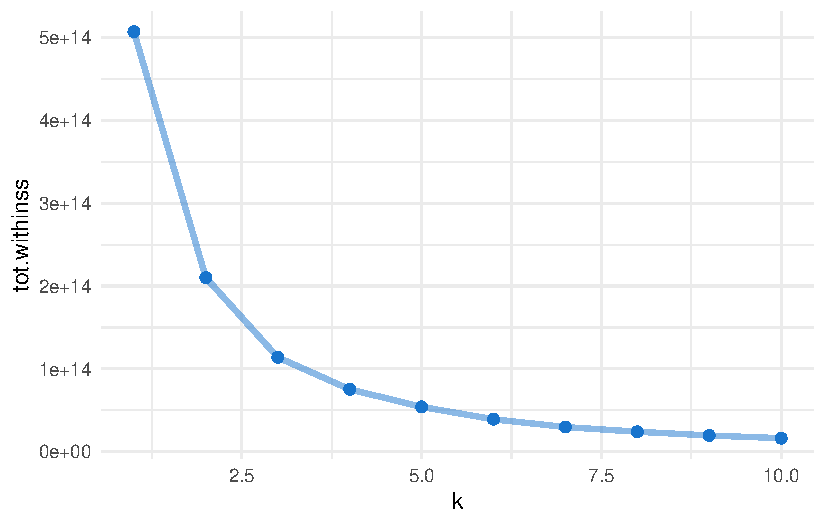
\includegraphics{k-means_final_files/figure-pdf/unnamed-chunk-3-1.pdf}

}

\end{figure}

\begin{Shaded}
\begin{Highlighting}[]
\FunctionTok{set.seed}\NormalTok{(}\DecValTok{503}\NormalTok{)}
\CommentTok{\# Fit and predict clusters with k = 3}
\NormalTok{final\_kmeans }\OtherTok{\textless{}{-}} \FunctionTok{kmeans}\NormalTok{(income\_features, }\AttributeTok{centers =}\DecValTok{3}\NormalTok{, }\AttributeTok{nstart =} \DecValTok{100}\NormalTok{, }\AttributeTok{iter.max =} \DecValTok{1000}\NormalTok{)}

\CommentTok{\# Add cluster prediction to the data set}
\NormalTok{results }\OtherTok{\textless{}{-}} \FunctionTok{augment}\NormalTok{(final\_kmeans, income\_features)}

\NormalTok{results }\SpecialCharTok{\%\textgreater{}\%} 
  \FunctionTok{slice\_head}\NormalTok{(}\AttributeTok{n =} \DecValTok{5}\NormalTok{)}
\end{Highlighting}
\end{Shaded}

\begin{verbatim}
# A tibble: 5 x 105
    age fnlwgt educati~1 capit~2 capit~3 hours~4 workc~5 workc~6 workc~7 workc~8
  <dbl>  <dbl>     <dbl>   <dbl>   <dbl>   <dbl>   <int>   <int>   <int>   <int>
1    25 226802         7       0       0      40       0       0       1       0
2    38  89814         9       0       0      50       0       0       1       0
3    28 336951        12       0       0      40       0       1       0       0
4    44 160323        10    7688       0      40       0       0       1       0
5    34 198693         6       0       0      30       0       0       1       0
# ... with 95 more variables: workclass_self_emp_not_inc <int>,
#   workclass_state_gov <int>, workclass_without_pay <int>,
#   `education_1st-4th` <int>, `education_5th-6th` <int>,
#   `education_7th-8th` <int>, education_9th <int>, education_10th <int>,
#   education_11th <int>, education_12th <int>, `education_Assoc-acdm` <int>,
#   `education_Assoc-voc` <int>, education_Bachelors <int>,
#   education_Doctorate <int>, `education_HS-grad` <int>, ...
\end{verbatim}

\begin{Shaded}
\begin{Highlighting}[]
\NormalTok{results }\OtherTok{\textless{}{-}} \FunctionTok{bind\_cols}\NormalTok{(}\FunctionTok{select}\NormalTok{(income, income\_above\_50k), }\FunctionTok{as.data.frame}\NormalTok{(results))}
\end{Highlighting}
\end{Shaded}

\begin{Shaded}
\begin{Highlighting}[]
\NormalTok{clust\_spc\_plot }\OtherTok{\textless{}{-}}\NormalTok{ results }\SpecialCharTok{\%\textgreater{}\%} 
    \FunctionTok{ggplot}\NormalTok{(}\AttributeTok{mapping =} \FunctionTok{aes}\NormalTok{(}\AttributeTok{x =}\NormalTok{ age, }\AttributeTok{y =}\NormalTok{ fnlwgt)) }\SpecialCharTok{+}
    \FunctionTok{geom\_point}\NormalTok{(}\FunctionTok{aes}\NormalTok{(}\AttributeTok{shape =}\NormalTok{ .cluster, }\AttributeTok{color=}\NormalTok{ .cluster),}\AttributeTok{size =} \DecValTok{2}\NormalTok{,}\AttributeTok{alpha=}\FloatTok{0.3}\NormalTok{)}\SpecialCharTok{+} 

  \FunctionTok{scale\_color\_manual}\NormalTok{(}\AttributeTok{values =} \FunctionTok{c}\NormalTok{(}\StringTok{"darkorange"}\NormalTok{,}\StringTok{"purple"}\NormalTok{,}\StringTok{"cyan4"}\NormalTok{))}\SpecialCharTok{+} \FunctionTok{theme\_minimal}\NormalTok{()}

\CommentTok{\# Make plot interactive}
\FunctionTok{ggplotly}\NormalTok{(clust\_spc\_plot)}
\end{Highlighting}
\end{Shaded}

\begin{itemize}
\tightlist
\item
  discussion for choosing number of clusters
\item
  analysis of cluster centers
\item
  bivariate chart(s) against meaningful variables and/or analysis of
  density plots
\item
  meaningful interpretation / discussion of conclusions
\end{itemize}



\end{document}
